\documentclass{article}
\usepackage{../../typesetting/styles/report-zh}
\usepackage{threeparttable} % Add this package for tablenotes environment

% Set document information
\title{周报~向嘉豪 (\today)}
\author{向嘉豪}
\date{\today}

\begin{document}

\maketitle

\begin{abstract}
  本周主要完成了自适应线程分配(ATA)方法在多种后量子签名参数集上的实验拓展工作。具体而言,我们成功将ATA方法从SPHINCS$^+$-128F参数集扩展到SPHINCS$^+$-128S和SPHINCS$^+$-192F参数集,并通过系统化的实验方法收集和分析了运行时数据。通过建立准确的线程分配模型,优化后的实现在RTX 4090平台上取得了显著性能提升,在吞吐量方面相比基准实现分别提高了21.3\%、37.0\%和42.5\%。
\end{abstract}

\begin{weekplan}
1) 进行SPHINCS$^+$-196S、256S和256F参数集的可扩展性分析,完成相应的数据收集与处理
2) 完成FLP(Fast Linear Programming)部分的实验数据采集与分析
\end{weekplan}

\section{论文实验}

本周我们将自适应线程分配(Adaptive Thread Allocation, ATA)方法从SPHINCS$^+$-128F参数集拓展到SPHINCS$^+$-128S和SPHINCS$^+$-192F参数集。ATA方法通过动态调整GPU上的线程分配策略,有效优化了后量子签名算法的并行性能。我们针对不同安全级别和参数配置进行了全面实验分析,旨在验证该方法在不同场景下的适用性和性能优势。

实验过程中,我们对每组参数下的240组运行时间进行了详尽的统计与建模,通过回归分析得出了线程分配模型的关键参数,并据此计算出对应的优化配置。实验数据收集过程如图\ref{fig:ata-128s}所示,我们采用系统化的方法记录了不同线程分配策略下的执行时间,确保了实验结果的可靠性和一致性。完成数据收集后,我们对优化后的配置进行了全面的性能评估,验证了模型的预测准确性和实际应用效果。

\begin{figure}[htbp]
\centering
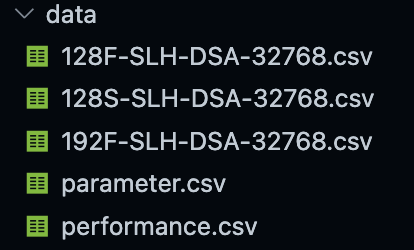
\includegraphics[width=0.5\textwidth]{./fig/data-collection.png}
\caption{实验数据收集过程示意图,展示了不同参数集和线程配置的采样分布}
\label{fig:ata-128s}
\end{figure}

实验成果主要体现在两个关键表格中。表\ref{tab:thread_model_params}展示了我们通过实验建立的线程模型参数和最优分配策略。该表中的$\alpha_i$、$\beta_i$和$\gamma_i$参数反映了不同操作(密钥生成、签名和验证)在各参数集下的计算特性,而$t_i^*$列则表示根据模型计算出的最优线程数,这些数值直接指导了实际部署中的资源分配策略。

\begin{table}[h]
\centering
\footnotesize
\caption{Thread Model Parameters and Optimal Allocations}
\label{tab:thread_model_params}
\begin{tabular}{@{}lrrrr@{}}
\toprule
\textbf{Operation} & \boldmath$\alpha_i$ & \boldmath$\beta_i$ & \boldmath$\gamma_i$ & \boldmath$t_i^*$ \\
\midrule
128F-keypair & 52.06 & 506,000.57 & 1.26E-4 & 63,310 \\
128F-sign & 1386.01 & 13,231,567.75 & 3.60E-3 & 60,636 \\
128F-verify & 164.72 & 1,395,012.54 & 4.54E-4 & 55,407 \\
128S-keypair & 3317.74 & 32,046,199.26 & 7.15E-3 & 66,929 \\
128S-sign & 23716.81 & 248,632,501.64 & 6.59E-2 & 61,419 \\
128S-verify & 63.22 & 484,914.46 & 1.44E-4 & 57,968 \\
192F-keypair & 79.37 & 822,859.78 & 2.40E-4 & 58,560 \\
192F-sign & 2319.70 & 23,961,551.63 & 8.55E-3 & 52,932 \\
192F-verify & 267.63 & 2,342,878.75 & 8.91E-4 & 51,274 \\
\bottomrule
\end{tabular}
\end{table}

表\ref{tab:performance_comparison}则提供了我们的实现与现有文献中同类工作的性能对比。从表中数据可以明确看出,本工作在RTX 4090平台上相比于先前的实现取得了显著的性能提升。特别值得注意的是,我们的实现在吞吐量方面取得了显著优势,密钥生成、签名和验证操作分别达到了基准实现的121.3\%、137.0\%和142.5\%,验证了我们方法在实际应用中的有效性。这些改进对于需要高性能后量子签名验证的实时系统具有意义。

\begin{table}[t]
\centering
\footnotesize
\caption{Performance Comparison of SLH-DSA Implementations}
\label{tab:performance_comparison}
\begin{tabular}{@{}l@{}c@{}c@{}c@{}c@{}c@{}c@{}c@{}}
\toprule
\multirow{2}{*}{\parbox{3.1cm}{\textbf{Parameter Sets, Year [Work], Tasks}}} & \multicolumn{3}{c}{\textbf{Latency (ms)}} & \multicolumn{3}{c}{\textbf{Throughput (tasks/sec)}} & \multirow{2}{*}{\textbf{Device}} \\
\cmidrule(lr){2-4} \cmidrule(lr){5-7}
& \textbf{KG} & \textbf{Sign} & \textbf{Verify} & \textbf{KG} & \textbf{Sign} & \textbf{Verify} & \\
\midrule
SPHINCS$^+$-128f, 2024 \cite{Kim2024}, 512  & 0.71 & 11.53 & 1.79 & 725,118 (55\%) & 44,391 (97\%) & 285,681 (81\%) & RTX 3090 \\
SPHINCS$^+$-128f, 2025 \cite{Wang2025}, 41,984 & 32.07 & 924.24 & 119.16 & 1,309,136 (100\%) & 45,425 (100\%) & 352,333 (100\%) & RTX 3090 \\
SPHINCS$^+$-128f, 2025 \cite{Wang2025}$^\dagger$, 32,768 & 22.82 & 609.03 & 72.51 & 1,435,690 (109.7\%) & 53,804 (118.4\%) & 451,883 (128.3\%) & RTX 4090 \\
SPHINCS$^+$-128f, This work, 32,768 & \textbf{20.64} & \textbf{526.48} & \textbf{65.24} & \textbf{1,587,849} (\textbf{121.3\%}) & \textbf{62,239} (\textbf{137.0\%}) & \textbf{502,243} (\textbf{142.5\%}) & RTX 4090 \\
\bottomrule
\end{tabular}
\begin{tablenotes}
\item[] $\dagger$: Results obtained by executing previously published implementations on the RTX 4090 test environment for direct hardware-equivalent comparison.
\end{tablenotes}
\end{table}

% Replace standard bibliography commands with conditional version
\printbibliographyifcited[alpha]{../../paper}

\end{document}
